\section{Zielsetzung}
\label{sec: Zielsetzung}
Ziel dieses Versuches ist es die Verdampfungswärme und die Dampfdruckkurve für Wasser zu bestimmen. 
Dazu wird der Vorgang der Phasenumwandlung von Wasser untersucht.

\section{Theorie}
\label{sec:Theorie}
\subsection{Allgemein} % (fold)
\label{sub:Allgemein}
Mit dem Begriff "Phase" werden, im Zusammenhang mit der Verdampfungswärme, räumlich abgegrenzte Bereiche in einem abgeschlossenen System bezeichnet.
Der Stoff, auf den sich bezogen wird, muss in einem physikalisch homogenen Zustand sein. 
Ein Beispiel für die Phase sind die Aggregatzustände (fest, flüssig und gasförmig), welche in einem Zustandsdiagramm aufgetragen sind.
\begin{figure}[H]
    \centering
    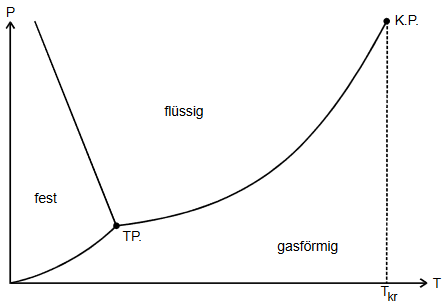
\includegraphics[width=0.5\textwidth]{build/Abb_1.PNG}
    \caption {Qualitatives Zustandsdiagramm von Wasser.\cite{v203}}
    \label{fig:Abb_1}
\end{figure}
In \autoref{fig:Abb_1} ist ein Zustandsdiagramm von Wasser zu sehen, wobei der Druck $p$ gegen die Temperatur $T$ aufgetragen ist.
Die Aggregatzustände sind in "Bereiche" abgegrenzt, wobei jeder Bereich die zwei Freiheitsgrade $p$ und $T$ besitzt.
Dies verändert sich jedoch in der Nähe der Kurven. 
Beim Trippelpunkt $TP$ gibt es keinen Freiheitsgrad, weil alle drei Aggregatzustände koexistieren.
In diesem Versuch wird nur die Dampfdruckkurve, also die Kurve zwischen den Punkt $TP$ und $KP$ betrachtet.
Auf der Dampfdruckkurve ist einem gewählten $T$ ein festgelegtes $p$ zugeordnet, weswegen es auf der Kurve nur einen Freiheitsgerad gibt. Die Kurve wird charakterisiert durch die Verdampfungswärme $L$.
Die Verdampfungswärme verschwindet in der Nähe des kritischen Punkts $KP$.
% subsection Allgemein (end)

\subsection{Mikroskopische Vorgänge bei der Verdampfung und Kondensation} % (fold)
\label{sub:Mikro_Vorgänge}
Bei einer Flüssigkeit in einem evakuierten Gefäß verdampft ein Teil der Flüssigkeit, was zu einem Druckanstieg führt.
Verdampfung allgemein entsteht dadurch, dass Moleküle die Flüssigkeitsmenge verlassen, wenn ihre kinetische Energie maximal ist.
Dafür muss Energie hinzugefügt werde, die molare Verdampfungswärme $L$.
Der Druck entsteht durch Bewegung der Gasmoleküle gegen die Gefäßwand und Flüssigkeit, wobei ein paar Moleküle wieder von der Flüssigkeit eingefangen werden.
Nach einer bestimmten Zeit und konstanten Bedingungen stellt sich ein Gleichgewichtszustand ein, wo der Nettostrom beinahe null ist und der Druck konstant ist.
Dieser Druck wird auch Sättigungsdampfdruck genannt, welcher mit zunehmender Temperatur ansteigt.
Er ist somit temperaturabhängig, aber nicht volumenabhängig.
Das Verhalten lässt sich jedoch nicht durch die allgemeine Gasgleichung
\begin{equation*}
    pV = RT
\end{equation*}
ausdrücken.

% subsection Mikroskopische Vorgänge (end)
 
\subsection{Die Clausius-Clapeyronsche Gleichung} % (fold)
\label{sub:CC-Gl}
Im folgenden wird die Clausius-Clapeyronsche Gleichung hergeleitet und erklärt. 
Diese Formel kann für eine System, wie oben beschrieben, benutzt werden.
Sie wird durch einen reversiblen Kreisprozess gewonnen, bei dem erst ein Mol eines Stoffes isotherm und isobar verdampft und ebenso kondensiert.
\begin{figure}[H]
    \centering
    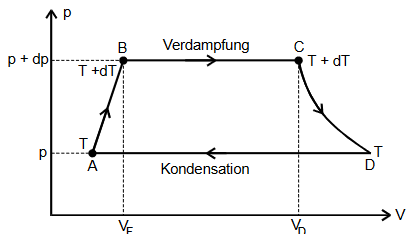
\includegraphics[width=0.5\textwidth]{build/Abb_2.PNG}
    \caption {Kreisprozess im pV-Diagramm, bei dem ein Stoff verdampft und wieder kondensiert.\cite{v203}}
    \label{fig:Abb_2}
\end{figure}
Ein Beispiel für so ein Kreisprozess ist in \autoref{fig:Abb_2} dargestellt und der Startzustand ist bei A, bei dem nur Flüssigkeit vorhanden ist.
Es wird eine Wärmemenge $dQ_{AB}$ zugeführt, weshalb der Druck und die Temperatur erhöht wird und es somit in den Zustand B übergeht.
Um in Zustand C zu gelangen, wird die Flüssigkeit isotherm und isobar verdampft, nachdem die Verdampfungswärme $L$ hinzugeführt wird.
In diesem Zustand ist nur Dampf vorhanden mit dem Volumen $V_D$.
Der vorliegende Dampf wird abgekühlt auf die Temperatur $T$, sodass Zustand D erreicht wird.
Durch Zufuhr mechanischer Energie kondensiert der Dampf und der Augsgangszustand A wird erreicht.
Die summierte Wärmemenge ergibt sich zu
\begin{equation}
    dQ_{ges} = C_F dT \,-\, C_D dt \,+\, L(T) \,+\, dL \,-\, L(T),
    \label{eqn:Wärmemenge}
\end{equation}
wobei $C_F$ die Molwärme der Flüssigkeit ist und $C_D$ die Molwärme des dampfes ist.
Die Wärmemenge wird gleichgesetzt mit der ganzen geleisteten Arbeit
\begin{equation}
    A = dp(V_D-V_F)
    \label{eqn:Arbeit}
\end{equation}
und dies wird umgeformt zu
\begin{equation}
    (V_D\,-\,V_F)dp = \frac{L}{T}dt .
    \label{eqn:CC-Gl}
\end{equation}
Diese Gleichung wird auch Clausius-Clapeyronsche Gleichung genannt. 
Die Integration ist kompliziert, jedoch können es in manchen Temperaturbereichen Nähreungsannamen getroffen werden, sodass die Integration leicht möglich ist.
Diese werden im nächsten Kapitel benannt.

% subsection CC-Gl (end)

\subsection{Annahmen zur Vereinfachung der Integration} % (fold)
\label{sub:Vereinfachung}
Die Temperatur $T$ liegt weit unter der kritischen Temperatur $T_{Kr}$ und $V_F$ ist gegenüber $V_D$ vernachlässigbar.
Wobei $V_D$ der idealen Gasgleichung
\begin{equation*}
    V_D(p,T) = R\frac{T}{p}
\end{equation*}
gehorcht.
Eine weitere Annahme ist, dass $L$ druck- und temperaturabhängig ist. 
Unter diesen Annahmen kann \autoref{eqn:CC-Gl} umgeformt werden und nach Integration fo,gt daraus
\begin{align}
    \text{ln}(p) &= -\frac{L}{RT}+const &\text{oder} && p=p_0 \text{exp}(-\frac{L}{RT})
    \label{eqn:CC-Gl_2}
\end{align}
% subsection Annahmen zur Vereinfachung der Integration (end)
 